\documentclass[12pt,a4paper]{article}
% Adapted from the SGU Assignment_report.tex template supplied by the user.
% Compile with pdfLaTeX from this directory.
\usepackage[utf8]{inputenc}
\usepackage[T5]{fontenc}
\usepackage[utf8]{vntex}
\usepackage[margin=2.3cm,top=2.8cm,bottom=2.6cm,headheight=40pt]{geometry}
\usepackage{graphicx,array,longtable,tabularx,booktabs,multirow}
\usepackage{amsmath,amssymb}
\usepackage{fancyhdr,lastpage,setspace,enumitem,float}
\usepackage[table]{xcolor}
\usepackage{tikz}
\usetikzlibrary{arrows.meta,positioning,fit,shapes.geometric,calc,backgrounds}
\usepackage{caption,xurl}
\usepackage{hyperref}
\hypersetup{colorlinks=true,linkcolor=black,urlcolor=blue,citecolor=black,
 pdftitle={BrewLite -- Báo cáo Assignment 1},pdfauthor={Nhóm sinh viên -- Chưa cung cấp}}
\graphicspath{{assets/}}
\setstretch{1.15}
\setlength{\parindent}{0pt}
\setlength{\parskip}{5pt}
\setlength{\emergencystretch}{3em}
\renewcommand{\arraystretch}{1.2}
\setlength{\tabcolsep}{5pt}
\setlist{nosep,leftmargin=*}
\captionsetup{font=small,labelfont=bf}
\setcounter{tocdepth}{2}
\newcolumntype{Y}{>{\raggedright\arraybackslash}X}

% Fill these fields when the group's information is available.
\newcommand{\GroupName}{Chưa cung cấp}
\newcommand{\LecturerName}{Chưa cung cấp}
\newcommand{\ClassName}{Chưa cung cấp}

\pagestyle{fancy}
\fancyhf{}
\fancyhead[L]{\begin{tabular}{@{}cl@{}}

\includegraphics[width=8mm]{logoITSGUsmall.png}&
\begin{tabular}{@{}l@{}}\small\textbf{Trường Đại học Sài Gòn}\\
\small Khoa Công nghệ Thông tin\end{tabular}\end{tabular}}
\fancyhead[R]{\small BrewLite\\Assignment 1}
\fancyfoot[L]{\scriptsize Công nghệ Phần mềm -- Học kỳ I, 2026--2027}
\fancyfoot[R]{\scriptsize Trang \thepage/\pageref{LastPage}}
\renewcommand{\headrulewidth}{0.3pt}
\renewcommand{\footrulewidth}{0.3pt}

\begin{document}
\begin{titlepage}
\centering
{\large\textbf{TRƯỜNG ĐẠI HỌC SÀI GÒN}}\\[4pt]
{\large\textbf{KHOA CÔNG NGHỆ THÔNG TIN}}
\vspace{1.1cm}


\includegraphics[width=3cm]{logoITSGU.png}
\vspace{1cm}

{\Large\textbf{CÔNG NGHỆ PHẦN MỀM}}\\[12pt]
\rule{\textwidth}{0.7pt}\\[12pt]
{\Huge\bfseries BrewLite}\\[12pt]
{\Large Hệ thống đặt cà phê không dùng tiền mặt}\\[12pt]
{\Large\textbf{BÁO CÁO ASSIGNMENT 1}}\\[8pt]
{\large Use Case -- User Story -- Kiến trúc hệ thống}\\[12pt]
\rule{\textwidth}{0.7pt}
\vspace{1cm}

\begin{tabular}{ll}
Giảng viên hướng dẫn: & \LecturerName\\
Nhóm: & \GroupName\\
Lớp: & \ClassName\\
Học kỳ: & I -- Năm học 2026--2027
\end{tabular}
\vspace{0.7cm}

\begin{tabularx}{0.85\textwidth}{@{}cYY@{}}
\toprule
STT & Họ và tên thành viên & MSSV\\\midrule
1 & Chưa cung cấp & Chưa cung cấp\\
\bottomrule
\end{tabularx}
\vfill
{\small TP. HỒ CHÍ MINH, THÁNG 11 NĂM 2026}
\end{titlepage}

\pagenumbering{roman}
\section*{Phạm vi báo cáo}
Tài liệu trình bày phân tích yêu cầu, User Story, Use Case và kiến trúc của
BrewLite theo đề \emph{BrewLite VER 1.0 -- Assignment 1}, gồm 10 task.
Luồng cốt lõi là xem menu, chọn size/topping, quản lý giỏ hàng, đăng nhập,
tạo đơn, thanh toán mô phỏng và xem xác nhận/lịch sử đơn.

Nội dung thiết kế được đối chiếu với mã nguồn trong repository. Các chức năng
quản trị, quản lý nguyên liệu và ZaloPay Sandbox được nhận diện là phần mở rộng.
Yêu cầu nghiệp vụ là tiêu chí để nghiệm thu; việc tìm thấy mã nguồn hoặc test
không tự đồng nghĩa tiêu chí đó đã được nghiệm thu đạt.
Kế hoạch Sprint trong báo cáo là đề xuất tổ chức công việc, không phải biên bản
các sự kiện Scrum đã diễn ra. Thông tin cá nhân chưa được cung cấp được để trống
bằng nhãn ``Chưa cung cấp''.

\tableofcontents
\clearpage
\pagenumbering{arabic}
\section{User Stories và yêu cầu nghiệm thu}
\label{sec:user-stories}

\subsection{Bối cảnh và phạm vi}
BrewLite là ứng dụng web giúp khách hàng chọn đồ uống, tùy chỉnh món, đặt hàng và thanh toán không dùng tiền mặt. Khách hàng là người dùng chính; quản lý cửa hàng/Product Owner ưu tiên backlog và nghiệm thu increment; nhân viên quầy/barista cập nhật trạng thái pha chế ở phần mở rộng; đơn vị thanh toán được mô phỏng bằng cổng ví/thẻ. Phạm vi MVP đi từ menu đến thanh toán và xác nhận đơn. Các yêu cầu FR-07--FR-10 là nghiệp vụ backend bổ sung trong Task 10 của đề Assignment 1.

Các story dưới đây mô tả yêu cầu và tiêu chí nghiệm thu, không phải báo cáo kết quả kiểm thử. Snapshot mã nguồn hiện có các module/API hoặc thành phần giao diện cho menu, chi tiết sản phẩm, giỏ hàng, xác thực, đơn hàng, thanh toán, lịch sử, state machine, idempotency, kiểm soát nguyên liệu, khuyến mãi và loyalty. Giỏ hàng hiện dùng localStorage/React state; đề bài nêu Zustand/Context như lựa chọn triển khai. Product Backlog và phân bổ Sprint bên dưới là kế hoạch đề xuất theo đề bài; chúng không khẳng định task đã hoàn tất, các sự kiện Scrum đã diễn ra, hay velocity thực tế đã được đo.

\subsection{Product Backlog yêu cầu}
Mỗi yêu cầu chức năng được liên kết với story và use case (UC) tương ứng. UC IDs được dùng theo danh mục use case của tài liệu.

\begin{longtable}{@{}p{1.3cm}p{1.9cm}p{2.2cm}p{2.1cm}p{6.8cm}@{}}
\caption{Ánh xạ yêu cầu, user story và use case}\label{tab:story-traceability}\\
\toprule
FR & Feature & User Story & Use Case & Phạm vi nghiệm thu chính \\
\midrule
\endfirsthead
\toprule FR & Feature & User Story & Use Case & Phạm vi nghiệm thu chính \\
\midrule
\endhead
\bottomrule
\endfoot
FR-01 & Menu & US-01 & \hyperref[uc01]{UC-01} & Danh sách đồ uống và thông tin cơ bản \\
FR-02 & Chi tiết & US-02 & \hyperref[uc02]{UC-02} & Chi tiết món, size, topping và giá \\
FR-03 & Giỏ hàng & US-03 & \hyperref[uc03]{UC-03} & Thêm, sửa, xóa món và tính tổng \\
FR-04 & Xác thực & US-04 & \hyperref[uc04]{UC-04} & Đăng ký, đăng nhập và bảo vệ thao tác đặt hàng \\
FR-05 & Đặt hàng, thanh toán & US-05, US-06 & \hyperref[uc06]{UC-06}; \hyperref[uc05]{UC-05} & Thanh toán không tiền mặt và tạo đơn \\
FR-06 & Xác nhận, lịch sử & US-07 & \hyperref[uc07]{UC-07} & Xác nhận sau thanh toán và xem lịch sử của khách \\
FR-07 & Vòng đời đơn & US-08 & \hyperref[uc08]{UC-08} & Chuyển trạng thái hợp lệ và từ chối chuyển sai \\
FR-08 & Chống lặp & US-09 & \hyperref[uc06]{UC-06} & Yêu cầu thanh toán lặp không tạo tác động lặp \\
FR-09 & Tồn kho nguyên liệu & US-10 & \hyperref[uc05]{UC-05} & Đặt đồng thời không bán vượt tồn kho \\
FR-10 & Khuyến mãi, loyalty & US-11 & \hyperref[uc05]{UC-05}; \hyperref[uc06]{UC-06} & Tính giảm giá và cộng điểm sau khi thanh toán \\
\end{longtable}

\subsection{User Stories và Acceptance Criteria}

\paragraph{US-01 -- Xem menu (FR-01).}
Là khách hàng, tôi muốn xem danh sách đồ uống kèm hình ảnh, tên và giá để chọn món phù hợp. Use case: \hyperref[uc01]{UC-01}.
\begin{enumerate}[label=\textbf{AC\arabic*:},leftmargin=*]
  \item Khi mở menu, hệ thống hiển thị các món đang bán với hình, tên và giá.
  \item Khi dữ liệu đang tải hoặc danh sách rỗng, giao diện hiển thị trạng thái tải hoặc thông báo chưa có món.
  \item Khi tải menu thất bại, giao diện báo lỗi và cho phép khách thử tải lại.
\end{enumerate}

\paragraph{US-02 -- Xem và tùy chỉnh món (FR-02).}
Là khách hàng, tôi muốn xem chi tiết đồ uống và chọn size/topping để biết giá món theo lựa chọn. Use case: \hyperref[uc02]{UC-02}.
\begin{enumerate}[label=\textbf{AC\arabic*:},leftmargin=*]
  \item Khi mở một món hợp lệ, hệ thống hiển thị thông tin và các lựa chọn size/topping được hỗ trợ.
  \item Khi thay đổi lựa chọn, giá đơn vị được tính lại bằng giá cơ bản, phụ thu size và giá topping đã chọn.
  \item Khi món không tồn tại hoặc lựa chọn không được hỗ trợ, hệ thống từ chối lựa chọn và thông báo lỗi.
\end{enumerate}

\paragraph{US-03 -- Quản lý giỏ hàng (FR-03).}
Là khách hàng, tôi muốn thêm, sửa hoặc xóa món trong giỏ để xem đúng các món và tổng tiền trước khi đặt. Use case: \hyperref[uc03]{UC-03}.
\begin{enumerate}[label=\textbf{AC\arabic*:},leftmargin=*]
  \item Khi thêm món, giỏ lưu sản phẩm, size, topping và số lượng; dòng có cùng sản phẩm và tùy chọn được gộp.
  \item Khi tăng/giảm số lượng hoặc xóa món, số lượng, badge giỏ hàng và tổng tiền được cập nhật; dòng được bỏ khi bị xóa.
  \item Khi giỏ rỗng, giao diện hiển thị trạng thái giỏ rỗng và không cho bắt đầu thanh toán.
\end{enumerate}

\paragraph{US-04 -- Đăng ký và đăng nhập (FR-04).}
Là khách hàng, tôi muốn tạo tài khoản và đăng nhập để đặt hàng gắn với tài khoản của mình. Use case: \hyperref[uc04]{UC-04}.
\begin{enumerate}[label=\textbf{AC\arabic*:},leftmargin=*]
  \item Khi gửi thông tin hợp lệ để đăng ký, hệ thống tạo tài khoản và không lưu mật khẩu dạng rõ.
  \item Khi đăng nhập thành công, hệ thống cấp JWT; dữ liệu sai hoặc không hợp lệ bị từ chối.
  \item Khi khách chưa xác thực gọi thao tác cần đăng nhập như đặt đơn, hệ thống từ chối yêu cầu.
\end{enumerate}

\paragraph{US-05 -- Thanh toán không tiền mặt (FR-05).}
Là khách hàng, tôi muốn thanh toán đơn bằng ví điện tử hoặc thẻ để không cần dùng tiền mặt. Use case: \hyperref[uc06]{UC-06}. Story này theo US-05 mẫu trong đề Assignment 1.
\begin{enumerate}[label=\textbf{AC\arabic*:},leftmargin=*]
  \item Khi giỏ có ít nhất một món, thao tác thanh toán hiển thị tổng tiền; khách có thể chọn Ví hoặc Thẻ.
  \item Khi cổng thanh toán báo lỗi, giao dịch ghi nhận thất bại, đơn ở trạng thái PAYMENT\_FAILED và giỏ hàng được giữ nguyên.
  \item Khi cổng thanh toán báo thành công, đơn chuyển sang PAID và giao diện hiển thị mã đơn cùng xác nhận. Giỏ tương ứng được xóa nếu vẫn khớp với đơn đã trả tiền; không xóa giỏ đã được khách sửa sau đó.
  \item Khi khách thử lại sau một lần thanh toán thất bại, yêu cầu mới dùng Idempotency-Key mới.
\end{enumerate}

\paragraph{US-06 -- Tạo đơn hàng (FR-05).}
Là khách hàng đã đăng nhập, tôi muốn tạo đơn từ giỏ hàng để hệ thống ghi nhận món và trả mã đơn. Use case: \hyperref[uc05]{UC-05}.
\begin{enumerate}[label=\textbf{AC\arabic*:},leftmargin=*]
  \item Khi gửi giỏ hợp lệ, hệ thống tự tính lại giá từ dữ liệu sản phẩm, lưu đơn ở trạng thái PENDING và trả mã đơn.
  \item Khi giỏ rỗng hoặc dữ liệu món, size, số lượng không hợp lệ, hệ thống từ chối và không tạo đơn.
  \item Đơn được gắn với tài khoản từ phiên xác thực; hệ thống không tin user ID hay giá do trình duyệt gửi lên.
\end{enumerate}

\paragraph{US-07 -- Xem xác nhận và lịch sử đơn (FR-06).}
Là khách hàng, tôi muốn xem xác nhận sau khi thanh toán và tra cứu các đơn trước đó để theo dõi giao dịch. Use case: \hyperref[uc07]{UC-07}.
\begin{enumerate}[label=\textbf{AC\arabic*:},leftmargin=*]
  \item Sau khi thanh toán thành công, màn hình xác nhận hiển thị mã đơn, trạng thái PAID và số tiền cuối cùng.
  \item Khi xem lịch sử, hệ thống chỉ trả các đơn thuộc tài khoản đang đăng nhập.
\end{enumerate}

\paragraph{US-08 -- Theo dõi vòng đời đơn (FR-07).}
Là quản lý cửa hàng, tôi muốn hệ thống chỉ cho phép các chuyển trạng thái hợp lệ để bảo toàn tiến trình đơn hàng. Use case: \hyperref[uc08]{UC-08}. Giao diện quản trị cập nhật trạng thái là phần mở rộng; phạm vi Assignment 1 yêu cầu nghiệp vụ state machine.
\begin{enumerate}[label=\textbf{AC\arabic*:},leftmargin=*]
  \item Hệ thống chấp nhận chuỗi PENDING $\rightarrow$ PAID $\rightarrow$ PREPARING $\rightarrow$ READY $\rightarrow$ COMPLETED; PAYMENT\_FAILED có thể trở lại PENDING để thử thanh toán lại.
  \item Khi yêu cầu chuyển trạng thái không có trong sơ đồ, hệ thống từ chối và giữ nguyên trạng thái hiện tại.
  \item COMPLETED và CANCELLED là trạng thái kết thúc, không chuyển tiếp sang trạng thái khác.
\end{enumerate}

\paragraph{US-09 -- Xử lý thanh toán lặp an toàn (FR-08).}
Là khách hàng, tôi muốn gửi lại yêu cầu khi mạng lỗi mà không bị tính tiền hoặc xử lý đơn hai lần. Use case: \hyperref[uc06]{UC-06}.
\begin{enumerate}[label=\textbf{AC\arabic*:},leftmargin=*]
  \item Khi cùng Idempotency-Key và cùng nội dung được gửi lại sau khi giao dịch hoàn tất, hệ thống trả kết quả đã lưu và chỉ ghi nhận một lần xử lý thanh toán.
  \item Khi cùng key được dùng với nội dung khác, hệ thống từ chối yêu cầu xung đột.
  \item Hai yêu cầu đồng thời cùng key không tạo xử lý thứ hai. Yêu cầu còn lại nhận kết quả đã hoàn tất; nếu giao dịch còn PENDING, hệ thống có thể trả 409 và yêu cầu thử lại với cùng key.
\end{enumerate}

\paragraph{US-10 -- Ngăn bán vượt tồn kho (FR-09).}
Là quản lý cửa hàng, tôi muốn việc đặt đồng thời được kiểm soát theo tồn kho nguyên liệu để không nhận đơn vượt khả năng phục vụ. Use case: \hyperref[uc05]{UC-05}.
\begin{enumerate}[label=\textbf{AC\arabic*:},leftmargin=*]
  \item Khi nhiều đơn đồng thời cần nguyên liệu chỉ còn đủ cho một đơn, tối đa một đơn được tạo thành công; các đơn còn lại bị từ chối do thiếu tồn.
  \item Sau các yêu cầu đồng thời, tồn kho không âm và chỉ thay đổi cùng giao dịch tạo đơn thành công.
\end{enumerate}

\paragraph{US-11 -- Dùng khuyến mãi và tích điểm (FR-10).}
Là khách hàng, tôi muốn áp mã giảm giá hợp lệ và nhận điểm sau khi thanh toán để được hưởng quyền lợi thành viên. Use case: \hyperref[uc05]{UC-05} và \hyperref[uc06]{UC-06}.
\begin{enumerate}[label=\textbf{AC\arabic*:},leftmargin=*]
  \item Khi mã còn hiệu lực và đơn đạt giá trị tối thiểu, hệ thống tính discount và số tiền cuối; mã không tồn tại, hết hạn hoặc không đủ điều kiện bị từ chối.
  \item Khi đơn chuyển sang PAID, khách nhận 1 điểm cho mỗi 1.000 đồng số tiền cuối, làm tròn xuống; mỗi đơn chỉ được cộng điểm một lần.
  \item Đơn chưa PAID hoặc thanh toán thất bại không được cộng điểm.
\end{enumerate}

\subsection{Yêu cầu phi chức năng}
\begin{itemize}[leftmargin=*]
  \item \textbf{Hiệu năng:} với dữ liệu mẫu, thời gian phản hồi API mục tiêu nhỏ hơn 500 ms cho menu, chi tiết sản phẩm, tạo đơn, thanh toán, lịch sử và xác thực. Đây là tiêu chí cần đo khi kiểm thử, không phải kết quả đã đo.
  \item \textbf{Bảo mật:} mật khẩu phải được băm; route đặt hàng cần JWT hợp lệ; dữ liệu đầu vào phải được kiểm tra và response không làm lộ password hash.
  \item \textbf{Tương thích:} luồng MVP phải hoạt động trên các trình duyệt web phổ biến đã thống nhất trong kế hoạch kiểm thử.
\end{itemize}

\subsection{Definition of Done}
Một task chỉ được xem là đạt Definition of Done khi thỏa các điều kiện trong Assignment 1:
\begin{itemize}[leftmargin=*]
  \item Mã nguồn chạy được, không lỗi build và đáp ứng tiêu chí chấp nhận của task.
  \item Có commit với thông điệp rõ ràng và được review trong nhóm.
  \item API kiểm tra dữ liệu đầu vào; giao diện xử lý tối thiểu trạng thái loading và lỗi.
  \item README có hướng dẫn thiết lập và chạy dự án.
\end{itemize}
Đây là tiêu chí nghiệm thu đề xuất; mục này không khẳng định task nào đã hoàn tất.

\subsection{Product Backlog và kế hoạch Sprint đề xuất}
Đề Assignment 1 quy định 10 task, mỗi task 1 điểm, tổng 10 điểm. Bảng dưới giữ nguyên phạm vi task; cách diễn đạt được rút gọn để truy vết với các story ở trên.

\begin{longtable}{@{}p{0.55cm}p{3.15cm}p{9.9cm}p{1.05cm}@{}}
\caption{Product Backlog Assignment 1}\label{tab:a1-product-backlog}\\
\toprule
\# & Task & Tiêu chí đầu ra & Điểm \\
\midrule
\endfirsthead
\toprule \# & Task & Tiêu chí đầu ra & Điểm \\
\midrule
\endhead
\bottomrule
\endfoot
1 & Khởi tạo dự án và cấu trúc & Tạo monorepo hoặc cấu trúc gồm frontend Next.js và backend NestJS chạy được; có Git, README và tệp cấu hình môi trường mẫu. & 1 \\
2 & API danh sách sản phẩm & API menu trả về ID, tên, giá và ảnh từ dữ liệu mẫu hoặc cơ sở dữ liệu. & 1 \\
3 & Trang Menu & Frontend gọi API sản phẩm, hiển thị danh sách cùng trạng thái tải và danh sách rỗng. & 1 \\
4 & Chi tiết và tùy chọn sản phẩm & Hiển thị chi tiết; chọn size/topping và tính giá theo lựa chọn. & 1 \\
5 & Giỏ hàng & Thêm, sửa số lượng, xóa; lưu trạng thái giỏ, tính tổng và hiển thị badge số lượng. & 1 \\
6 & API tạo đơn hàng & API kiểm tra dữ liệu, lưu đơn PENDING và trả mã đơn. & 1 \\
7 & Đăng ký/đăng nhập (JWT) & Đăng ký, đăng nhập, băm mật khẩu, cấp JWT và bảo vệ route đặt đơn. & 1 \\
8 & Thanh toán không tiền mặt & Chọn Ví/Thẻ; tích hợp ZaloPay Sandbox; đơn chuyển PAID khi thành công, PAYMENT\_FAILED khi lỗi. & 1 \\
9 & Xác nhận, lịch sử và bàn giao & Màn hình xác nhận, API lịch sử; Docker Compose chạy frontend/backend/database; README và demo end-to-end. & 1 \\
10 & Nghiệp vụ backend & State machine, idempotency, chống bán vượt tồn kho khi đặt đồng thời, khuyến mãi và loyalty; có kiểm thử unit/integration cho tiêu chí Task 10. & 1 \\
\end{longtable}

\begin{table}[htbp]
\centering
\small
\begin{tabularx}{\textwidth}{@{}p{1.5cm}p{3.1cm}X@{}}
\toprule
Sprint đề xuất & Mục tiêu & Task \\
\midrule
Sprint 1 & Nền tảng và menu & Task 1, 2, 3, 4 \\
Sprint 2 & Giỏ hàng, đặt đơn và đăng nhập & Task 5, 6, 7 \\
Sprint 3 & Thanh toán, bàn giao và nghiệp vụ nâng cao & Task 8, 9, 10 \\
\bottomrule
\end{tabularx}
\caption{Phân bổ ba Sprint được đề xuất trong Assignment 1. Đây là kế hoạch tham khảo, không phải lịch sử Sprint đã thực hiện.}
\label{tab:a1-sprint-plan}
\end{table}

\clearpage
\section{Phân tích Use Case}
\label{sec:use-cases}

\subsection{Phạm vi và tác nhân}

BrewLite hỗ trợ khách hàng chọn đồ uống, tùy chỉnh món, quản lý giỏ hàng,
đăng nhập, tạo đơn và thanh toán không dùng tiền mặt để nhận tại quầy.
Phần này trình bày mô hình ca sử dụng của Assignment~1. Các đặc tả tập trung
vào hành vi quan sát được và điều kiện chấp nhận; việc có mã nguồn tương ứng
không đồng nghĩa mọi điều kiện đã được kiểm thử hoặc hệ thống đã sẵn sàng
vận hành thanh toán thật.

Luồng khách hàng UC-01--UC-07 là trọng tâm MVP. Quản trị đơn hàng ở UC-08,
quản lý nguyên liệu theo công thức và tích hợp ZaloPay Sandbox được ghi nhận
là phần mở rộng hiện có trong mã nguồn. Chúng giúp làm rõ cách thực thi
quy tắc nghiệp vụ, không thay thế phạm vi MVP bằng một hệ thống quản trị đầy đủ.

\begin{longtable}{|p{3.0cm}|p{11.6cm}|}
\caption{Tác nhân và trách nhiệm trong mô hình Use Case}
\label{tab:uc-actors}\\ \hline
\textbf{Tác nhân} & \textbf{Vai trò} \\ \hline
\endfirsthead
\hline \textbf{Tác nhân} & \textbf{Vai trò} \\ \hline
\endhead
Khách hàng & Xem menu khi chưa đăng nhập; chọn món và lưu giỏ trong trình
duyệt; xác thực trước khi tạo đơn, thanh toán hoặc xem dữ liệu đơn cá nhân. \\ \hline
Quản trị viên & Tác nhân của phần mở rộng: xem đơn của cửa hàng, cập nhật
tiến độ pha chế và hủy đơn còn đủ điều kiện. Phải được xác thực và có quyền
quản trị; không phải mọi khách hàng đã đăng nhập đều có quyền này. \\ \hline
Cổng thanh toán & Hệ thống bên ngoài cung cấp kết quả thanh toán. Trong
MVP, cổng giả lập đóng vai trò mô phỏng phụ thuộc này; phần mở rộng sử dụng
ZaloPay Sandbox. Không có giao dịch tiền thật trong luồng thử nghiệm. \\ \hline
\end{longtable}

Backend, cơ sở dữ liệu, bộ xác thực JWT và tác vụ định kỳ là thành phần
nội bộ của BrewLite, không được mô hình hóa thành tác nhân bên ngoài.

\subsection{Sơ đồ Use Case tổng quát}

\begin{figure}[htbp]
\centering
\begin{tikzpicture}[
  x=1cm,y=1cm,font=\small,
  uc/.style={ellipse,draw,align=center,text width=5.5cm,
    minimum height=0.96cm,inner sep=3pt},
  actorlabel/.style={align=center,text width=2.5cm,font=\small}
]
  \draw[rounded corners=2pt] (2.1,0.9) rectangle (10.8,-11.8);
  \node[font=\bfseries] at (6.45,0.5) {Hệ thống BrewLite};
  \node[uc] (uc01) at (6.45,-0.5) {UC-01: Xem và tìm món};
  \node[uc] (uc02) at (6.45,-2.0) {UC-02: Xem chi tiết, chọn tùy chọn};
  \node[uc] (uc03) at (6.45,-3.5) {UC-03: Quản lý giỏ hàng};
  \node[uc] (uc04) at (6.45,-5.0) {UC-04: Đăng ký, đăng nhập};
  \node[uc] (uc05) at (6.45,-6.5) {UC-05: Tạo đơn hàng};
  \node[uc] (uc06) at (6.45,-8.0) {UC-06: Thanh toán đơn hàng};
  \node[uc] (uc07) at (6.45,-9.5) {UC-07: Xem xác nhận và lịch sử};
  \node[uc,dashed] (uc08) at (6.45,-11.0) {UC-08: Xử lý trạng thái đơn\\(mở rộng quản trị)};
  % UML actors are drawn directly to keep the report self-contained.
  \draw (0.8,-4.1) circle (0.18);
  \draw (0.8,-4.28)--(0.8,-4.95);
  \draw (0.35,-4.55)--(1.25,-4.55);
  \draw (0.8,-4.95)--(0.4,-5.45) (0.8,-4.95)--(1.2,-5.45);
  \node[actorlabel] at (0.8,-5.8) {Khách hàng};
  \coordinate (customer) at (1.3,-4.55);
  \foreach \target in {uc01,uc02,uc03,uc04,uc05,uc06,uc07}
    \draw (customer)--(\target.west);
  \draw (12.0,-7.1) circle (0.18);
  \draw (12.0,-7.28)--(12.0,-7.95);
  \draw (11.55,-7.55)--(12.45,-7.55);
  \draw (12.0,-7.95)--(11.6,-8.45) (12.0,-7.95)--(12.4,-8.45);
  \node[actorlabel] at (12.0,-8.9) {Cổng thanh toán};
  \draw (11.55,-7.55)--(uc06.east);
  \draw (12.0,-9.8) circle (0.18);
  \draw (12.0,-9.98)--(12.0,-10.65);
  \draw (11.55,-10.25)--(12.45,-10.25);
  \draw (12.0,-10.65)--(11.6,-11.15) (12.0,-10.65)--(12.4,-11.15);
  \node[actorlabel] at (12.0,-11.65) {Quản trị viên};
  \draw (11.55,-10.25)--(uc08.east);
\end{tikzpicture}
\caption{Các mục tiêu sử dụng BrewLite và ranh giới hệ thống}
\label{fig:overall-use-case}
\end{figure}

Đường nối trong Hình~\ref{fig:overall-use-case} biểu diễn sự tham gia của
tác nhân, không biểu diễn thứ tự thao tác. Xác thực là tiền điều kiện của
các ca sử dụng được bảo vệ; khách hàng có phiên hợp lệ không cần thực hiện
lại UC-04 mỗi khi tạo đơn. Quy tắc trạng thái được dùng chung trong
UC-05--UC-08; UC-08 thể hiện riêng mục tiêu vận hành của quản trị viên.

\subsection{Danh mục và truy vết yêu cầu}

\begin{longtable}{|p{1.3cm}|p{3.6cm}|p{6.3cm}|p{2.7cm}|}
\caption{Danh mục Use Case và liên kết yêu cầu chức năng}
\label{tab:uc-catalog}\\ \hline
\textbf{Mã} & \textbf{Tên} & \textbf{Kết quả mong muốn} & \textbf{Yêu cầu} \\ \hline
\endfirsthead
\hline \textbf{Mã} & \textbf{Tên} & \textbf{Kết quả mong muốn} & \textbf{Yêu cầu} \\ \hline
\endhead
UC-01 & Xem và tìm món & Có danh sách món, giá, ảnh, danh mục và tình trạng
phục vụ; tìm kiếm, lọc theo danh mục. & FR-01 \\ \hline
UC-02 & Chi tiết và tùy chọn & Chọn size, topping được hỗ trợ, số lượng và
xem giá tạm tính trước khi thêm giỏ. & FR-02 \\ \hline
UC-03 & Quản lý giỏ hàng & Xem, sửa, xóa món; cập nhật tổng tạm tính và
chuyển sang đặt hàng. & FR-03 \\ \hline
UC-04 & Đăng ký, đăng nhập & Nhận phiên xác thực để thực hiện giao dịch và
truy cập dữ liệu cá nhân. & FR-04 \\ \hline
UC-05 & Tạo đơn hàng & Có mã đơn, giá đã xác nhận và trạng thái chờ thanh
toán; giữ tồn kho, áp dụng ưu đãi hợp lệ. & FR-05, FR-07, FR-09, FR-10 \\ \hline
UC-06 & Thanh toán đơn hàng & Ghi nhận kết quả thanh toán nhất quán,
không tạo giao dịch trùng khi gửi lại cùng yêu cầu. & FR-05, FR-07, FR-08, FR-10 \\ \hline
UC-07 & Xác nhận và lịch sử & Xem mã nhận món, nội dung đơn, tổng tiền,
trạng thái và lịch sử đơn của bản thân. & FR-06, FR-07 \\ \hline
UC-08 & Xử lý trạng thái đơn & Quản trị viên cập nhật tiến độ hợp lệ và có
dấu vết thay đổi; hủy đơn theo quy tắc. & FR-07, FR-09, FR-10; mở rộng \\ \hline
\end{longtable}

Trong bảng trên, FR-07 là máy trạng thái đơn; FR-08 là tính lũy đẳng
thanh toán; FR-09 là xử lý tồn kho khi có truy cập đồng thời; FR-10 là
khuyến mãi và tích điểm. Các yêu cầu này là quy tắc xuyên suốt nhiều ca
sử dụng, không buộc khách hàng phải thao tác với một màn hình riêng.

\subsection{Đặc tả UC-01: Xem và tìm món}
\label{uc:01}
\label{uc01}

\begin{longtable}{|p{3.1cm}|p{11.5cm}|}
\hline \textbf{Thuộc tính} & \textbf{Nội dung} \\ \hline
Tác nhân, kích hoạt & Khách hàng mở trang menu hoặc thay đổi từ khóa,
danh mục. \\ \hline
Tiền điều kiện & Truy cập được ứng dụng; không bắt buộc đăng nhập. \\ \hline
Hậu điều kiện & Hiển thị danh sách phù hợp hoặc trạng thái rỗng/lỗi rõ
ràng; chưa tạo đơn hay thay đổi tồn kho. \\ \hline
Liên kết & FR-01; chuyển sang UC-02 khi chọn món. \\ \hline
\end{longtable}

\textbf{Luồng chính}
\begin{enumerate}[nosep]
  \item Khách hàng mở \path{/menu}; hệ thống hiển thị trạng thái đang tải.
  \item Hệ thống lấy danh sách qua \path{GET /api/v1/products} và hiển thị
  tên, ảnh, giá cơ bản, danh mục, tình trạng phục vụ.
  \item Khách hàng nhập từ khóa hoặc chọn danh mục.
  \item Giao diện lọc kết hợp hai điều kiện trên danh sách đã tải; khách
  hàng chọn món để xem chi tiết hoặc mở hộp chọn tùy chọn.
\end{enumerate}

\textbf{Thay thế và ngoại lệ.} Danh sách chưa có món được hiển thị bằng
trạng thái rỗng. Không có kết quả tìm kiếm/lọc được thông báo riêng. Khi
lỗi mạng, giao diện báo lỗi và cho phép thử lại. Món không khả dụng vẫn
có thể xuất hiện với nhãn hết hàng và nút mua bị khóa; không suy diễn rằng
mọi món hiển thị đều chắc chắn còn nguyên liệu tại thời điểm đặt đơn.

\textbf{Điều kiện chấp nhận.} Kết quả kết hợp đúng từ khóa và danh mục;
tìm tên không phân biệt hoa/thường và bỏ khoảng trắng đầu/cuối. Mã hiện
tại chưa chuẩn hóa dấu tiếng Việt, vì vậy tìm không dấu chưa được coi là
tiêu chí đã đáp ứng. Nút mua không hoạt động với món hết hàng hoặc chưa có
size khả dụng.

\subsection{Đặc tả UC-02: Xem chi tiết và chọn tùy chọn}
\label{uc:02}
\label{uc02}

\begin{longtable}{|p{3.1cm}|p{11.5cm}|}
\hline \textbf{Thuộc tính} & \textbf{Nội dung} \\ \hline
Tác nhân, kích hoạt & Khách hàng chọn một món trong menu hoặc mở trang
chi tiết món. \\ \hline
Tiền điều kiện & Có định danh sản phẩm hợp lệ; để thêm giỏ, món và size
phải đang khả dụng. \\ \hline
Hậu điều kiện & Dòng món với cấu hình đã chọn được lưu vào giỏ của trình
duyệt; nếu thao tác thất bại, không thêm dòng không hợp lệ. \\ \hline
Liên kết & FR-02; dữ liệu được dùng tiếp bởi UC-03 và xác minh lại tại UC-05. \\ \hline
\end{longtable}

\textbf{Luồng chính}
\begin{enumerate}[nosep]
  \item Hệ thống lấy chi tiết qua \path{GET /api/v1/products/:id}.
  \item Khách hàng xem thông tin món và chọn size trong các size được hỗ trợ.
  \item Với đồ uống ngoài nhóm cà phê, khách hàng có thể chọn tối đa ba
  loại topping khả dụng, không trùng lặp. Cà phê chỉ chọn size, không dùng topping.
  \item Khách hàng chọn số lượng từ 1 đến 99; giao diện cập nhật giá tạm tính.
  \item Khách hàng xác nhận; hệ thống thêm cấu hình vào giỏ và thông báo kết quả.
\end{enumerate}

\textbf{Thay thế và ngoại lệ.} Khi sửa một dòng trong giỏ, cấu hình mới
thay thế dòng được chọn. Không có topping khả dụng thì khách hàng vẫn có
thể mua món không topping. Món không tồn tại, lỗi tải, size hết hàng hoặc
dữ liệu giá không hợp lệ phải được thông báo; không cho thêm món khi chưa
có cấu hình hợp lệ. Nếu nguyên liệu thay đổi sau lúc xem chi tiết, kết
quả cuối cùng được quyết định tại UC-05.

\textbf{Điều kiện chấp nhận.} Giá hiển thị cho một dòng bằng số lượng
nhân với tổng giá cơ bản, phụ thu size và giá topping. Cấu hình cà phê
không chứa topping; các giới hạn số lượng và topping được kiểm tra lại ở
backend khi tạo đơn. Giá trong trình duyệt là ước tính, không phải giá
được backend tin cậy.

\subsection{Đặc tả UC-03: Quản lý giỏ hàng}
\label{uc:03}
\label{uc03}

\begin{longtable}{|p{3.1cm}|p{11.5cm}|}
\hline \textbf{Thuộc tính} & \textbf{Nội dung} \\ \hline
Tác nhân, kích hoạt & Khách hàng mở giỏ, sửa cấu hình, tăng/giảm số lượng
hoặc xóa một món. \\ \hline
Tiền điều kiện & Có thể mở giỏ khi chưa đăng nhập; có dòng món nếu muốn
sửa, xóa hoặc tiếp tục đặt hàng. \\ \hline
Hậu điều kiện & Giỏ trong trình duyệt và tổng tạm tính được cập nhật;
chưa trừ tồn kho và chưa ghi nhận thanh toán. \\ \hline
Liên kết & FR-03; UC-04 nếu cần đăng nhập, sau đó UC-05. \\ \hline
\end{longtable}

\textbf{Luồng chính}
\begin{enumerate}[nosep]
  \item Khách hàng mở \path{/cart}; hệ thống nạp giỏ đã lưu trong trình duyệt.
  \item Hệ thống trình bày tên món, size, topping, số lượng và thành tiền tạm tính.
  \item Khách hàng chỉnh số lượng hoặc cấu hình; các dòng cùng sản phẩm,
  size và cùng tập topping được gộp theo quy tắc của giỏ.
  \item Hệ thống lưu thay đổi và tính lại tổng tiền.
  \item Khách hàng xác nhận các món để chuyển sang bước đặt hàng.
\end{enumerate}

\textbf{Thay thế và ngoại lệ.} Khách hàng xóa dòng không còn cần; xóa hết
thì hiển thị giỏ rỗng và không tiếp tục checkout. Số lượng ngoài giới hạn
không được chấp nhận. Nếu chưa đăng nhập, khách hàng được yêu cầu xác
thực trước khi đặt hàng. Giỏ hiện tại của giao diện khách hàng dùng
\texttt{localStorage}; các API Cart có trong backend không phải bằng
chứng về đồng bộ giỏ đa thiết bị của giao diện này.

\textbf{Điều kiện chấp nhận.} Sửa/xóa cập nhật ngay giỏ và tổng tiền; hai
cấu hình khác size hoặc khác tập topping không bị gộp nhầm. Không cho gửi
đơn với giỏ rỗng; backend giới hạn tối đa 50 dòng trong một yêu cầu tạo đơn.

\subsection{Đặc tả UC-04: Đăng ký và đăng nhập}
\label{uc:04}
\label{uc04}

\begin{longtable}{|p{3.1cm}|p{11.5cm}|}
\hline \textbf{Thuộc tính} & \textbf{Nội dung} \\ \hline
Tác nhân, kích hoạt & Khách hàng chọn đăng ký/đăng nhập hoặc cần thực hiện
một thao tác được bảo vệ. \\ \hline
Tiền điều kiện & Chưa có phiên hợp lệ; để đăng nhập cần tài khoản đã tồn tại. \\ \hline
Hậu điều kiện & Thành công: có JWT và thông tin người dùng. Thất bại:
không cấp phiên cho thông tin sai hoặc dữ liệu không hợp lệ. \\ \hline
Liên kết & FR-04; tiền điều kiện của UC-05--UC-07 và truy cập quản trị. \\ \hline
\end{longtable}

\textbf{Luồng chính: đăng nhập}
\begin{enumerate}[nosep]
  \item Khách hàng mở biểu mẫu, nhập email và mật khẩu.
  \item Giao diện gửi \path{POST /api/v1/auth/login}.
  \item Backend kiểm tra dữ liệu, đối chiếu mật khẩu với giá trị đã băm.
  \item Hệ thống cấp JWT, trả thông tin tài khoản; giao diện cập nhật phiên.
  \item Khách hàng tiếp tục thao tác cần xác thực.
\end{enumerate}

\textbf{Luồng thay thế: đăng ký.} Khách hàng nhập họ tên, email, mật khẩu
và xác nhận mật khẩu. Giao diện gửi \path{POST /api/v1/auth/register};
backend kiểm tra dữ liệu và email duy nhất, lưu mật khẩu đã băm rồi cấp
phiên cho tài khoản mới. Điểm tích lũy ban đầu bằng không.

\textbf{Ngoại lệ.} Email đã dùng được báo xung đột; dữ liệu sai định dạng
được báo để sửa. Khi đăng nhập sai, hệ thống trả thông báo chung về thông
tin đăng nhập. JWT thiếu, hết hạn hoặc không hợp lệ không được truy cập
API bảo vệ; giao diện cần yêu cầu đăng nhập lại.

\textbf{Điều kiện chấp nhận.} Không trả mật khẩu hay giá trị băm cho client.
Đơn hàng cá nhân luôn gắn với người dùng được xác thực, không nhận danh
tính chủ đơn tùy ý từ trình duyệt. Có phiên đăng nhập không tự động cấp
quyền quản trị.

\subsection{Đặc tả UC-05: Tạo đơn hàng}
\label{uc:05}
\label{uc05}

\begin{longtable}{|p{3.1cm}|p{11.5cm}|}
\hline \textbf{Thuộc tính} & \textbf{Nội dung} \\ \hline
Tác nhân, kích hoạt & Khách hàng xác nhận đặt hàng tại trang checkout. \\ \hline
Tiền điều kiện & Phiên đăng nhập hợp lệ; giỏ từ 1 đến 50 dòng; mỗi dòng
chứa sản phẩm, size, topping và số lượng hợp lệ. \\ \hline
Hậu điều kiện & Thành công: có đơn \texttt{PENDING}, mã đơn, chi tiết và
giá đã xác nhận; nguyên liệu/topping được giữ bằng cách trừ kho, điểm sử
dụng được ghi nhận. Thất bại: giao dịch rollback, không lưu đơn dở dang
hoặc trừ kho/điểm một phần. \\ \hline
Liên kết & FR-05, FR-07, FR-09, FR-10; tiếp tục UC-06. \\ \hline
\end{longtable}

\textbf{Luồng chính}
\begin{enumerate}[nosep]
  \item Khách hàng xem món đã chọn, có thể nhập mã khuyến mãi và số điểm muốn dùng.
  \item Giao diện kiểm tra đơn đang chờ gắn với giỏ hiện tại để có thể tiếp
  tục đơn trước đó, sau đó gửi \path{POST /api/v1/orders} khi cần tạo đơn mới.
  Yêu cầu chỉ chứa cấu hình món và lựa chọn ưu đãi, không chứa giá được tin cậy.
  \item Backend xác thực người dùng, kiểm tra sản phẩm đang bán, size hỗ
  trợ, topping cho phép và tính lại toàn bộ giá từ cơ sở dữ liệu.
  \item Backend cộng nhu cầu nguyên liệu từ công thức theo sản phẩm, size
  và số lượng; kiểm tra và trừ nguyên liệu cùng topping trong giao dịch.
  \item Backend kiểm tra hiệu lực, điều kiện mã khuyến mãi và số dư điểm;
  tính số tiền cuối cùng, tạo đơn \texttt{PENDING}, lưu chi tiết và lịch sử trạng thái.
  \item Hệ thống trả mã đơn và số tiền đã xác nhận; giao diện lưu tham
  chiếu đơn đang chờ rồi chuyển đến trang thanh toán.
\end{enumerate}

\textbf{Luồng thay thế}
\begin{itemize}[nosep]
  \item Giỏ chưa thay đổi và đã có đơn \texttt{PENDING} hoặc
  \texttt{PAYMENT\_FAILED}: giao diện tiếp tục đơn đó. Nếu giỏ đã sửa, giao
  diện xử lý hủy đơn chờ cũ trước khi tạo đơn mới theo cơ chế hiện có.
  \item Không nhập mã hay không dùng điểm: tính đơn theo giá thông thường.
  Mã hợp lệ được áp dụng trước phần giảm bằng điểm.
  \item Điểm sử dụng là bội số của 10, mỗi điểm giảm 100~đồng; không vượt
  số dư và số tiền sau khuyến mãi. Điều kiện này được xác minh tại backend.
\end{itemize}

\textbf{Ngoại lệ.} Từ chối giỏ rỗng, sản phẩm không bán, size không có
công thức, topping không hợp lệ, mã ưu đãi không đủ điều kiện hoặc điểm
không đủ. Khi thiếu nguyên liệu hoặc dữ liệu tồn kho thay đổi đồng thời,
trả thông báo để khách tải lại/thử lại; không âm kho và không ghi đơn một phần.

\textbf{Điều kiện chấp nhận.} Tổng tiền do backend quyết định. Tồn kho
đồ uống được tính từ nguyên liệu của công thức theo size, không mô tả
bằng một trường tồn kho sản phẩm độc lập. Cập nhật nguyên liệu kiểm tra
\texttt{version} và số dư, kết hợp giao dịch \texttt{Serializable}; topping
được trừ có điều kiện đủ kho. Khi hai khách tranh lượng nguyên liệu cuối,
chỉ yêu cầu đáp ứng đủ điều kiện mới thành công, yêu cầu còn lại nhận lỗi
có thể xử lý. Cơ chế tiếp tục đơn ở giao diện không được suy rộng thành
cam kết lũy đẳng cho mọi yêu cầu tạo đơn từ client bất kỳ.

\subsection{Đặc tả UC-06: Thanh toán đơn hàng}
\label{uc:06}
\label{uc06}

\begin{longtable}{|p{3.1cm}|p{11.5cm}|}
\hline \textbf{Thuộc tính} & \textbf{Nội dung} \\ \hline
Tác nhân, kích hoạt & Khách hàng chọn phương thức và xác nhận thanh toán;
cổng thanh toán cung cấp kết quả. \\ \hline
Tiền điều kiện & JWT hợp lệ; đơn thuộc khách hàng, đang ở
\texttt{PENDING} hoặc \texttt{PAYMENT\_FAILED}; không có giao dịch thành
công hoặc giao dịch đang xử lý khác chặn lần thanh toán này. \\ \hline
Hậu điều kiện & Thành công: Payment là \texttt{SUCCESS}, đơn là
\texttt{PAID}, điểm thưởng và lịch sử được ghi nhất quán. Thất bại:
Payment là \texttt{FAILED}, đơn là \texttt{PAYMENT\_FAILED}; có thể thử
lại bằng yêu cầu mới theo quy tắc. \\ \hline
Liên kết & FR-05, FR-07, FR-08, FR-10; kết quả được xem tại UC-07. \\ \hline
\end{longtable}

\textbf{Luồng chính của thanh toán giả lập trong MVP}
\begin{enumerate}[nosep]
  \item Hệ thống nạp đơn từ backend, hiển thị số tiền đã xác nhận; khách
  hàng chọn ví điện tử hoặc thẻ nội địa trong luồng mô phỏng.
  \item Giao diện gửi \path{POST /api/v1/payments} với mã đơn, phương thức
  và header \texttt{Idempotency-Key} cho lần thanh toán.
  \item Backend kiểm tra quyền sở hữu, trạng thái đơn, khóa lũy đẳng và
  dấu vân tay nội dung yêu cầu; số tiền lấy từ đơn trong cơ sở dữ liệu.
  \item Backend tuần tự hóa các lần thanh toán của cùng đơn bằng khóa
  hàng, tạo giao dịch và nhận kết quả từ cổng giả lập.
  \item Với kết quả thành công, backend cập nhật giao dịch và chuyển đơn
  sang \texttt{PAID} trong cùng giao dịch dữ liệu; ghi lịch sử và cộng
  $\lfloor\text{số tiền cuối cùng}/1000\rfloor$ điểm thưởng.
  \item Giao diện hiển thị kết quả. Chỉ xóa giỏ tương ứng với đơn đang
  chờ khi giỏ hiện tại còn khớp bản đã đặt, tránh xóa các món vừa sửa.
\end{enumerate}

\textbf{Luồng thay thế và ngoại lệ}
\begin{itemize}[nosep]
  \item Cổng giả lập trả thất bại: lưu \texttt{FAILED}, chuyển đơn sang
  \texttt{PAYMENT\_FAILED}; giữ thông tin để khách thử lại hoặc hủy đơn.
  Lần thử mới dùng khóa mới; khi thử lại đơn chuyển về \texttt{PENDING}.
  \item Gửi lại cùng khóa và cùng nội dung sau khi đã hoàn tất: trả kết
  quả đã lưu, không tạo Payment và không cộng điểm lần nữa. Khóa trùng
  nhưng nội dung khác bị từ chối với xung đột.
  \item Mất phản hồi hoặc còn đang xử lý: client giữ khóa của lần gửi
  đó để kiểm tra/gửi lại, không suy ra thất bại chỉ vì chưa thấy kết quả.
  Giao dịch cùng khóa còn \texttt{PENDING} có thể trả xung đột yêu cầu thử lại.
  \item Sai chủ đơn, đơn đã hủy/đã thanh toán hoặc có giao dịch khác đang
  xử lý: từ chối, không tạo lần thu tiền mới.
\end{itemize}

\textbf{Điều kiện chấp nhận.} Gửi lặp hoặc gửi đồng thời không ghi nhận
hai lần thanh toán thành công cho một đơn. Giao dịch và trạng thái đơn
không mâu thuẫn; điểm chỉ được thưởng khi chuyển hợp lệ sang
\texttt{PAID}. ZaloPay Sandbox chỉ hoạt động khi \texttt{NODE\_ENV} là
\texttt{development}/\texttt{test}, \texttt{ZALOPAY\_SANDBOX\_ENABLED=true}
và có đủ bộ khoá sandbox; không dùng tiền thật.

\textbf{Luồng ZaloPay Sandbox.} Mã nguồn có luồng tạo yêu cầu
\path{POST /api/v1/payments/zalopay}, nhận callback và đồng bộ kết quả.
Luồng này có trạng thái chờ bất đồng bộ; callback phải được kiểm tra
chữ ký và dữ liệu giao dịch trước khi cập nhật đơn. Giao diện kiểm tra
giao dịch Sandbox đang chờ trước khi cho tạo lượt mới. Cấu hình sandbox,
khả năng nhận callback và kiểm thử tích hợp là điều kiện triển khai riêng;
báo cáo không coi đây là thanh toán thật đã nghiệm thu.

\subsection{Đặc tả UC-07: Xem xác nhận và lịch sử đơn}
\label{uc:07}
\label{uc07}

\begin{longtable}{|p{3.1cm}|p{11.5cm}|}
\hline \textbf{Thuộc tính} & \textbf{Nội dung} \\ \hline
Tác nhân, kích hoạt & Khách hàng xem kết quả sau thanh toán, mở danh sách
đơn hoặc chọn một đơn cụ thể. \\ \hline
Tiền điều kiện & Phiên hợp lệ; đơn cần xem thuộc khách hàng hiện tại. \\ \hline
Hậu điều kiện & Hiển thị dữ liệu đơn được backend xác nhận; việc xem
không tự đổi trạng thái hoặc tạo giao dịch mới. \\ \hline
Liên kết & FR-06, FR-07; có thể quay lại UC-06 nếu đơn còn được thanh toán. \\ \hline
\end{longtable}

\textbf{Luồng chính}
\begin{enumerate}[nosep]
  \item Khách hàng mở \path{/orders}; hệ thống gọi \path{GET /api/v1/orders/me}.
  \item Hệ thống hiển thị danh sách đơn cá nhân, mã đơn, thời gian, số
  lượng món, tổng tiền và trạng thái; hỗ trợ phân trang và lọc trạng thái.
  \item Khách hàng chọn đơn; hệ thống gọi \path{GET /api/v1/orders/:id}.
  \item Giao diện trình bày món và tùy chọn, các khoản tiền, kết quả
  thanh toán, lịch sử trạng thái và mã đơn dùng khi nhận tại quầy.
\end{enumerate}

\textbf{Thay thế và ngoại lệ.} Chưa có đơn thì hiển thị lịch sử rỗng.
Đơn chưa thanh toán có thể tiếp tục UC-06. Đơn đủ điều kiện có thể được
khách hàng hủy bằng \path{POST /api/v1/orders/:id/cancel}; quy tắc hoàn
kho, điểm và hoàn tiền theo UC-08. Phiên hết hạn yêu cầu đăng nhập lại;
đơn không tồn tại hoặc không thuộc khách được báo không tìm thấy, không
trả dữ liệu đơn người khác. Lỗi tải có thông báo và khả năng thử lại.

\textbf{Điều kiện chấp nhận.} Danh sách và chi tiết chỉ chứa đơn thuộc
người được xác thực. Nhãn thành công dựa trên trạng thái do backend trả
về, không dựa riêng vào trang chuyển hướng của cổng thanh toán. Không
khẳng định có hóa đơn email, mã QR nhận món hay thông báo đẩy nếu chưa
có luồng tương ứng trong phạm vi.

\subsection{Đặc tả UC-08: Xử lý trạng thái đơn hàng (mở rộng)}
\label{uc:08}
\label{uc08}

\begin{longtable}{|p{3.1cm}|p{11.5cm}|}
\hline \textbf{Thuộc tính} & \textbf{Nội dung} \\ \hline
Tác nhân, kích hoạt & Quản trị viên mở danh sách đơn và xác nhận tiến độ
thực tế tại quầy. \\ \hline
Tiền điều kiện & Phiên hợp lệ, có quyền quản trị; đơn tồn tại và chuyển
trạng thái được phép. \\ \hline
Hậu điều kiện & Trạng thái, phiên bản và lịch sử đơn được cập nhật nhất
quán; thay đổi sai quy tắc bị từ chối. Khi hủy, hoàn kho/điểm theo quy tắc. \\ \hline
Liên kết & FR-07, FR-09, FR-10; phần quản trị là mở rộng của MVP. \\ \hline
\end{longtable}

\textbf{Luồng chính}
\begin{enumerate}[nosep]
  \item Quản trị viên mở danh sách/chi tiết đơn qua các API
  \path{/api/v1/admin/orders} được bảo vệ bằng JWT và quyền quản trị.
  \item Quản trị viên chọn hành động tương ứng với công việc đã thực hiện.
  \item Hệ thống kiểm tra trạng thái và phiên bản hiện tại, chỉ chấp nhận
  các bước \texttt{PAID} $\rightarrow$ \texttt{PREPARING}
  $\rightarrow$ \texttt{READY} $\rightarrow$ \texttt{COMPLETED}.
  \item Hệ thống lưu trạng thái mới cùng người thay đổi, thời điểm và lý
  do; giao diện khách hàng có thể đọc trạng thái mới khi tải lại dữ liệu.
\end{enumerate}

\textbf{Luồng thay thế: hủy đơn.} Khách hàng sở hữu đơn hoặc quản trị
viên được hủy khi đơn ở \texttt{PENDING}, \texttt{PAYMENT\_FAILED} hoặc
\texttt{PAID}, trước khi bắt đầu pha chế. Hệ thống chuyển sang
\texttt{CANCELLED}, hoàn đúng lượng nguyên liệu đã ghi với đơn, hoàn
topping và điểm đã sử dụng. Với đơn đã trả tiền, thu hồi điểm đã thưởng
và ghi \texttt{MANUAL\_REQUIRED}: tiền cần được hoàn thủ công, không có
cam kết hoàn tiền tự động. Gọi hủy lại đơn đã hủy không được hoàn kho/điểm lần hai.

\textbf{Tác vụ nội bộ hiện có.} Scheduler mỗi phút tìm đơn
\texttt{PENDING} được tạo hơn 15 phút để gọi cơ chế hủy và hoàn kho.
Quy tắc hiện tại không tự áp dụng cho \texttt{PAYMENT\_FAILED}; không
diễn giải thành việc hủy mọi đơn sau 15 phút, hay giữ món 15 phút sau thanh toán.

\textbf{Ngoại lệ và điều kiện chấp nhận.} Từ chối tài khoản không có
quyền, bỏ bước pha chế, quay lui trạng thái kết thúc hoặc hủy khi đã
\texttt{PREPARING}. Khi có cập nhật đồng thời, điều kiện phiên bản phải
ngăn ghi đè; người dùng nhận thông báo tải lại. Hủy phải qua nghiệp vụ
hủy có hoàn kho/điểm, không chỉ gán trực tiếp trạng thái.

\subsection{Quy tắc trạng thái và kiểm chứng chấp nhận}

\begin{longtable}{|p{3.1cm}|p{5.8cm}|p{5.2cm}|}
\caption{Các chuyển trạng thái được phép}
\label{tab:order-transitions}\\ \hline
\textbf{Trạng thái nguồn} & \textbf{Trạng thái đích} & \textbf{Sự kiện} \\ \hline
\endfirsthead
\hline \textbf{Trạng thái nguồn} & \textbf{Trạng thái đích} & \textbf{Sự kiện} \\ \hline
\endhead
Chưa có đơn & \texttt{PENDING} & Tạo đơn hợp lệ. \\ \hline
\texttt{PENDING} & \texttt{PAID}, \texttt{PAYMENT\_FAILED},
\texttt{CANCELLED} & Thanh toán thành công, thất bại hoặc hủy hợp lệ. \\ \hline
\texttt{PAYMENT\_FAILED} & \texttt{PENDING}, \texttt{CANCELLED} & Thử
thanh toán lại hoặc hủy. \\ \hline
\texttt{PAID} & \texttt{PREPARING}, \texttt{CANCELLED} & Bắt đầu pha
chế hoặc hủy trước pha chế; hủy cần hoàn tiền thủ công. \\ \hline
\texttt{PREPARING} & \texttt{READY} & Pha chế xong. \\ \hline
\texttt{READY} & \texttt{COMPLETED} & Đã giao đồ uống tại quầy. \\ \hline
\texttt{COMPLETED}, \texttt{CANCELLED} & Không có & Trạng thái kết thúc. \\ \hline
\end{longtable}

Những tình huống sau là cơ sở thiết kế kiểm thử và nghiệm thu, không phải
báo cáo kết quả chạy kiểm thử:
\begin{enumerate}[nosep]
  \item \textbf{Luồng mua hoàn chỉnh:} xem menu, chọn size/topping hợp
  lệ, thêm giỏ, đăng nhập, tạo đơn, thanh toán thành công và xem lại đúng
  đơn trong lịch sử (UC-01--UC-07; FR-01--FR-06).
  \item \textbf{Chuyển trạng thái sai:} thử chuyển
  \texttt{PAID} thẳng sang \texttt{READY}; hệ thống từ chối và giữ lịch
  sử nhất quán (UC-08; FR-07).
  \item \textbf{Thanh toán lặp:} gửi đồng thời cùng khóa/cùng nội dung;
  chỉ có một kết quả nghiệp vụ. Thử lại khóa đó với nội dung khác phải
  bị từ chối (UC-06; FR-08).
  \item \textbf{Tranh tồn kho:} hai khách cùng đặt lượng nguyên liệu
  cuối; kiểm tra không âm kho, đơn lỗi không để lại dữ liệu một phần và
  thông báo cho phép xử lý tiếp (UC-05; FR-09).
  \item \textbf{Ưu đãi và điểm:} mã hết hạn, chưa đạt mức tối thiểu,
  điểm vượt số dư hoặc không là bội số của 10 đều bị từ chối. Thanh toán
  lặp không thưởng điểm hai lần; hủy lặp không hoàn điểm hai lần
  (UC-05, UC-06, UC-08; FR-10).
  \item \textbf{Quyền truy cập:} khách A không xem/thanh toán đơn của
  khách B; tài khoản khách không cập nhật trạng thái qua API quản trị
  (UC-04, UC-06--UC-08).
\end{enumerate}

\subsection{Căn cứ và giới hạn của đặc tả}

Các ca sử dụng được tổng hợp từ đề Assignment~1
\path{BrewLite-CongNghePhanMem.pdf}, tài liệu các phân hệ trong
\path{docs/product-catalog}, \path{docs/product-detail}, \path{docs/cart},
\path{docs/auth}, \path{docs/order}, \path{docs/payment} và
\path{docs/order-history}. Hành vi cụ thể được đối chiếu với
\path{backend/src/modules/orders/orders.service.ts},
\path{backend/src/modules/orders/order-state.ts},
\path{backend/src/modules/products/products.service.ts},
\path{backend/src/modules/payments/zalopay-sandbox.service.ts},
\path{backend/src/modules/payments/zalopay-sandbox.gateway.ts},
\path{frontend/src/lib/pending-order.ts} và các trang giao diện liên quan.

Một số tài liệu phân hệ phản ánh thiết kế ở thời điểm cũ, ví dụ chỉ hiển
thị món còn hàng, tìm không dấu hoặc chưa có tác vụ hết hạn đơn. Khi mô
tả hiện trạng, phần này dùng hành vi trong mã nguồn đã đối chiếu và nêu
rõ phần mở rộng. Việc nghiệm thu cần thực thi các tình huống chấp nhận
trong môi trường cấu hình tương ứng, đặc biệt với xử lý đồng thời,
callback Sandbox và hoàn tiền thủ công.

\clearpage
\section{Thiết kế kiến trúc và công nghệ}
\label{sec:architecture}

\subsection{Phạm vi và hướng tổ chức}

BrewLite sử dụng kiến trúc phân lớp trong một monorepo: ứng dụng web Next.js gọi REST API NestJS; backend truy cập PostgreSQL thông qua Prisma. Đây là kiến trúc của Bài tập lớn 1, phục vụ luồng xem menu, chọn size/topping, giỏ hàng, đăng nhập, đặt đơn, thanh toán mô phỏng và tra cứu đơn. Các cơ chế trạng thái đơn, chống thanh toán lặp, giữ tồn kho và khuyến mãi/điểm thưởng là phần hiện thực nghiệp vụ Task 10 của cùng đề bài; việc đạt toàn bộ tiêu chí chấp nhận cần được xác nhận bằng kết quả kiểm thử.

Backend được tổ chức thành một ứng dụng theo module, không tách thành các microservice. Cách tổ chức này cho phép một transaction bao trùm đơn hàng, tồn kho và điểm thưởng trong cùng CSDL, đồng thời giữ việc chạy thử bằng Docker Compose đơn giản. Các sơ đồ dưới đây thể hiện cấu trúc đã có trong mã nguồn; phần mở rộng được ghi rõ để tránh nhầm với phạm vi MVP.

\begin{figure}[htbp]
\centering
\begin{tikzpicture}[
  box/.style={draw,rounded corners,align=center,inner sep=7pt,font=\small},
  flow/.style={-{Latex[length=2mm]},thick},
  note/.style={font=\scriptsize,align=center}]
  \node[box,text width=12.7cm] (ui) at (0,0) {\textbf{Lớp trình bày --- Next.js App Router}\\
  TypeScript, React, Tailwind CSS; menu, giỏ hàng, checkout, thanh toán, lịch sử đơn\\
  React state + localStorage; services + fetchApi gửi REST/JSON};
  \node[box,text width=12.7cm,below=0.8cm of ui] (api) {\textbf{Lớp HTTP --- NestJS Controllers}\\
  /api/v1; JWT Guard; DTO ValidationPipe; giới hạn yêu cầu\\
  TransformInterceptor chuẩn hóa kết quả; AllExceptionsFilter chuẩn hóa lỗi};
  \node[box,text width=8.9cm,anchor=north west] (biz) at ([yshift=-0.8cm]api.south west) {\textbf{Lớp nghiệp vụ --- NestJS Services}\\
  Auth, Products, Cart, Orders, Payments\\
  Mở rộng: Users, Ingredients, Recipes, StockImports\\
  State machine, giá/ưu đãi, transaction, kiểm soát đồng thời};
  \node[box,text width=2.35cm,right=0.5cm of biz] (zlp) {\textbf{ZaloPay Sandbox}\\Ví / Thẻ\\Dịch vụ ngoài\\HTTPS};
  \node[box,text width=8.9cm,below=0.8cm of biz] (data) {\textbf{Lớp dữ liệu --- PrismaService / Prisma Client}\\
  PostgreSQL: quan hệ, khóa ngoại, unique, transaction\\
  Schema + migrations + dữ liệu seed cho local/test};
  \draw[flow] (ui) -- node[right,note]{HTTP + Bearer JWT} (api);
  \draw[flow] (api.south -| biz.north) -- (biz.north);
  \draw[flow] (biz) -- (zlp);
  \draw[flow] (biz) -- (data);
\end{tikzpicture}
\caption{Kiến trúc phân lớp của BrewLite; ZaloPay Sandbox là dịch vụ ngoài, chỉ dùng ở mức thử nghiệm.}
\label{fig:layered-architecture}
\end{figure}

\subsection{Trách nhiệm của các thành phần}

\begin{longtable}{@{}p{0.21\linewidth}p{0.73\linewidth}@{}}
\toprule
\textbf{Thành phần} & \textbf{Trách nhiệm và ranh giới} \\
\midrule
\endfirsthead
\toprule
\textbf{Thành phần} & \textbf{Trách nhiệm và ranh giới} \\
\midrule
\endhead
Next.js / React & App Router định tuyến các trang; các trang tương tác sử dụng React hooks. Giỏ hàng nháp lưu ở \texttt{brewlite-cart} trong localStorage; JWT lưu ở \texttt{token}. Giá trên giao diện chỉ là ước tính, backend tính lại khi tạo đơn. \\
AuthModule & Đăng ký, đăng nhập, hồ sơ; bcrypt băm mật khẩu; Passport kiểm tra JWT và đối chiếu tài khoản, email, \texttt{tokenVersion} trong CSDL. \\
ProductsModule & Trả menu, chi tiết, danh mục và giá theo size; cung cấp dữ liệu nguồn cho UI. \\
CartModule & Có API và mô hình giỏ hàng lưu trong CSDL. Luồng giỏ hàng web hiện đọc/ghi localStorage; không mặc nhiên đồng bộ với CartModule. \\
OrdersModule & Tính tiền, kiểm tra ưu đãi và điểm sử dụng; giữ nguyên liệu/topping, tạo đơn; chuyển trạng thái, hủy/hoàn kho, trả lịch sử theo chủ đơn. \\
PaymentsModule & Xử lý lượt thanh toán, kiểm tra quyền sở hữu, idempotency và trạng thái giao dịch; tích hợp ZaloPay Sandbox qua create/callback/query/cancel và cung cấp màn hình quản lý thanh toán. \\
PrismaModule & Cung cấp PrismaService dùng chung, kết nối PostgreSQL và transaction; schema là nguồn định nghĩa quan hệ dữ liệu. \\
Module mở rộng & Users quản lý người dùng; Ingredients quản lý nguyên liệu; Recipes quản lý định mức; StockImports quản lý nhập kho. Những màn hình quản trị này hỗ trợ vận hành và minh họa nghiệp vụ, vượt tập màn hình khách hàng tối thiểu. \\
Config / Schedule & Đọc cấu hình môi trường; chạy tác vụ định kỳ kiểm tra đơn \texttt{PENDING} quá hạn. \\
\bottomrule
\end{longtable}

Nguồn đối chiếu: \path{backend/src/app.module.ts}, \path{frontend/src/app/checkout/page.tsx}, \path{frontend/src/app/cart/page.tsx}, \path{frontend/src/services/order.service.ts} và \path{frontend/src/lib/api-client.ts}. Gói Zustand có trong \path{frontend/package.json}, nhưng chưa thấy được import trong \path{frontend/src}; vì vậy báo cáo không mô tả giỏ hàng là một Zustand store đã hiện thực. Đây là điểm cần đối chiếu khi nghiệm thu Task 5, vì đề gợi ý lưu state bằng Zustand/Context.

\subsection{Vòng đời một yêu cầu và kiểm soát truy cập}

\begin{enumerate}[leftmargin=*,itemsep=3pt]
  \item UI gọi service, service dùng \texttt{fetchApi}. Wrapper gửi JSON qua header \texttt{Content-Type}; nếu có token, thêm header \texttt{Authorization} với giá trị \texttt{Bearer <token>}. URL gốc mặc định là \url{http://localhost:4000/api/v1}.
  \item NestJS định tuyến đến controller. Với API được bảo vệ, \texttt{JwtAuthGuard} kiểm tra chữ ký, hạn dùng và payload; \texttt{JwtStrategy} đối chiếu \texttt{sub}, email và \texttt{ver} với tài khoản hiện có. Đổi mật khẩu tăng \texttt{tokenVersion} để vô hiệu token cũ. Các API quản trị bổ sung kiểm tra vai trò ở backend.
  \item Interceptor giới hạn yêu cầu chạy trước handler; DTO qua \texttt{ValidationPipe} với \texttt{whitelist=true}, \texttt{forbidNonWhitelisted=true}, \texttt{transform=true}. Dữ liệu sai kiểu/ràng buộc hoặc trường ngoài DTO bị từ chối. Guard diễn ra trước pipe, nên JWT không hợp lệ có thể bị chặn trước lỗi DTO.
  \item Controller lấy người dùng từ JWT rồi gọi service. Service kiểm tra quyền sở hữu đơn và các quy tắc nghiệp vụ, thay vì tin \texttt{userId}, giá hoặc tổng tiền do trình duyệt tự khai báo. Prisma thực thi truy vấn/transaction theo yêu cầu của service.
  \item Thành công được bọc thành \texttt{success, statusCode, data, timestamp}. Lỗi đi qua \texttt{AllExceptionsFilter}, trả \texttt{success=false}, mã HTTP, \texttt{error}, \texttt{message}, thời điểm và đường dẫn. Frontend lấy \texttt{data} hoặc ném \texttt{ApiError} để trang hiển thị lỗi.
\end{enumerate}

Giới hạn yêu cầu hiện dùng Map trong bộ nhớ của một tiến trình: nhóm đọc tối đa 60 yêu cầu/phút theo danh tính, nhóm ghi một yêu cầu/5 giây theo danh tính và thao tác; phản hồi 429 có \texttt{Retry-After}. Đây không phải bộ giới hạn dùng chung giữa nhiều replica. JWT lưu trong localStorage thuận tiện cho demo nhưng có thể bị mã JavaScript đọc nếu xuất hiện XSS; cần đánh giá lại cơ chế phiên khi triển khai thật. Cấu hình CORS hiện phục vụ phát triển, chưa thể coi là cấu hình production đã siết chặt.

Nguồn: \path{backend/src/main.ts}, \path{backend/src/modules/auth/auth.service.ts}, \path{backend/src/modules/auth/jwt.strategy.ts}, \path{backend/src/common/guards/admin.guard.ts}, \path{backend/src/common/interceptors/request-limits.interceptor.ts}, \path{backend/src/common/interceptors/transform.interceptor.ts} và \path{backend/src/common/filters/http-exception.filter.ts}.

\subsection{Mô hình dữ liệu nghiệp vụ}

Schema hiện thực các thực thể tối thiểu trong đề và bổ sung thực thể cho tùy chọn món, kho, lịch sử trạng thái và loyalty. Tiền của sản phẩm, đơn và thanh toán lưu bằng \texttt{Decimal(12,0)} theo VNĐ; giá đơn được chốt tại lúc đặt, không lấy lại giá hiện tại khi thanh toán. Không nên suy rộng rằng mọi đại lượng trong CSDL đều là Decimal: tồn nguyên liệu và một số trường nhập kho hiện dùng Float.

\begin{longtable}{@{}p{0.27\linewidth}p{0.67\linewidth}@{}}
\toprule
\textbf{Thực thể / nhóm} & \textbf{Thuộc tính và quan hệ chính} \\
\midrule
\endfirsthead
\toprule
\textbf{Thực thể / nhóm} & \textbf{Thuộc tính và quan hệ chính} \\
\midrule
\endhead
User & Email unique, \texttt{passwordHash}, \texttt{tokenVersion}, vai trò, số dư điểm; một người có nhiều đơn và giao dịch loyalty. \\
Product, Category, ProductSizePrice & Product có tên, ảnh, giá gốc và cờ bán; mỗi cặp sản phẩm--size là duy nhất, chứa phụ thu. Danh mục của sản phẩm có thể để trống. \\
Order & Chủ đơn, mã số hiển thị unique, trạng thái, tổng tiền/giảm giá/thành tiền, \texttt{version}, thời điểm trả tiền và điểm đã cộng. Có thể gắn một Promotion. \\
OrderItem, OrderItemTopping, Topping & Dòng đơn giữ sản phẩm, size, số lượng, đơn giá và thành tiền; bảng nối topping giữ giá tại lúc đặt. Topping có tồn kho riêng. \\
Payment & Nhiều lượt thử cho một đơn; \texttt{idempotencyKey} unique toàn cục, hash nội dung, số tiền, phương thức, trạng thái và tham chiếu giao dịch ZaloPay. Trường nguồn giữ giá trị \texttt{MOCK} chỉ để đọc bản ghi lịch sử; giao dịch mới dùng \texttt{ZALOPAY\_SANDBOX}. \\
Promotion & Mã unique, mức giảm theo phần trăm hoặc số tiền, điều kiện giá trị tối thiểu, thời hạn và trạng thái kích hoạt. \\
LoyaltyTransaction & Sổ giao dịch điểm theo người dùng, có thể gắn đơn; loại \texttt{EARNED}, \texttt{SPENT}, \texttt{REFUNDED}, \texttt{REVERSED}, số điểm và lý do. \\
OrderStatusHistory & Ghi trạng thái trước/sau, tác nhân, lý do và thời điểm mỗi lần chuyển trạng thái. \\
Ingredient, RecipeIngredient, OrderIngredient & Công thức theo sản phẩm--size--nguyên liệu; lượng cần dùng; tồn và version nguyên liệu. OrderIngredient chốt lượng đã giữ cho đơn, phục vụ hoàn kho đúng lượng khi hủy. \\
Cart, CartItem & Giỏ lưu ở backend, quan hệ người dùng--giỏ là tùy chọn; CartItem có sản phẩm, size, số lượng và danh sách ID topping. Luồng web hiện sử dụng giỏ nháp ở trình duyệt. \\
StockImport, StockImportItem & Phần mở rộng nhập kho: phiếu nhập, nguyên liệu, số lượng, đơn giá, tổng tiền. \\
\bottomrule
\end{longtable}

\begin{figure}[htbp]
\centering
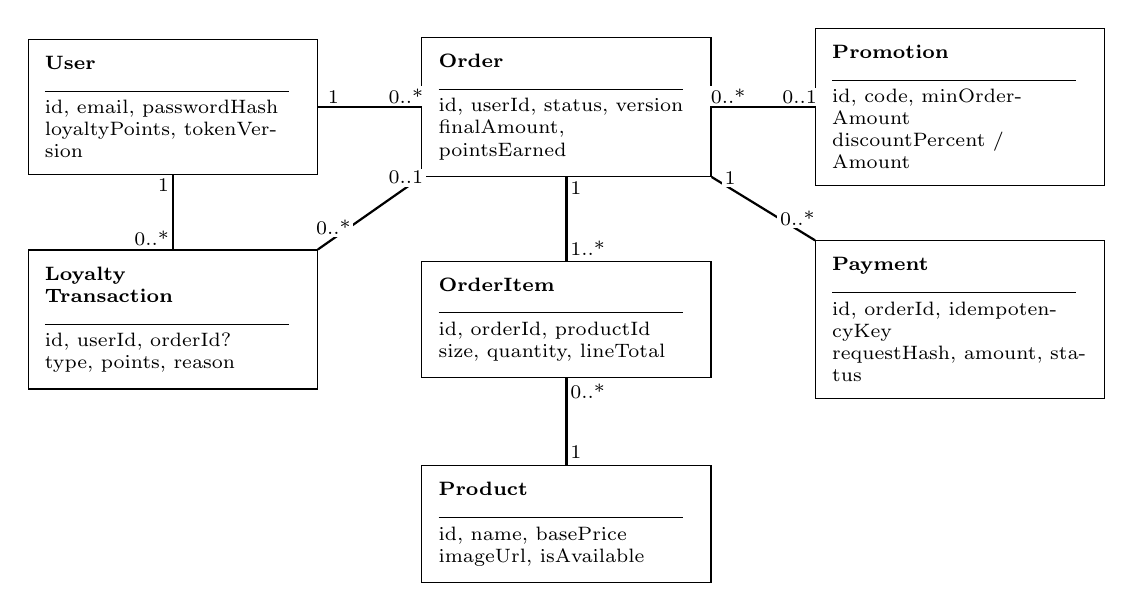
\begin{tikzpicture}[
  cls/.style={draw,rectangle,align=left,text width=3.25cm,inner sep=6pt,font=\scriptsize},
  rel/.style={thick}, mult/.style={font=\scriptsize,fill=white,inner sep=1pt}]
  \node[cls] (user) at (0,0) {\textbf{User}\\\rule{3.1cm}{0.3pt}\\id, email, passwordHash\\loyaltyPoints, tokenVersion};
  \node[cls] (order) at (5,0) {\textbf{Order}\\\rule{3.1cm}{0.3pt}\\id, userId, status, version\\finalAmount, pointsEarned};
  \node[cls] (promo) at (10,0) {\textbf{Promotion}\\\rule{3.1cm}{0.3pt}\\id, code, minOrderAmount\\discountPercent / Amount};
  \node[cls] (loyalty) at (0,-2.7) {\textbf{Loyalty}\\\textbf{Transaction}\\\rule{3.1cm}{0.3pt}\\id, userId, orderId?\\type, points, reason};
  \node[cls] (item) at (5,-2.7) {\textbf{OrderItem}\\\rule{3.1cm}{0.3pt}\\id, orderId, productId\\size, quantity, lineTotal};
  \node[cls] (payment) at (10,-2.7) {\textbf{Payment}\\\rule{3.1cm}{0.3pt}\\id, orderId, idempotencyKey\\requestHash, amount, status};
  \node[cls] (product) at (5,-5.3) {\textbf{Product}\\\rule{3.1cm}{0.3pt}\\id, name, basePrice\\imageUrl, isAvailable};
  \draw[rel] (user) -- node[mult,pos=.15,above]{1} node[mult,pos=.85,above]{0..*} (order);
  \draw[rel] (order) -- node[mult,pos=.16,above]{0..*} node[mult,pos=.85,above]{0..1} (promo);
  \draw[rel] (user) -- node[mult,pos=.14,left]{1} node[mult,pos=.85,left]{0..*} (loyalty);
  \draw[rel] (order) -- node[mult,pos=.14,right]{1} node[mult,pos=.85,right]{1..*} (item);
  \draw[rel] (order.south east) -- node[mult,pos=.18,above]{1} node[mult,pos=.83,above]{0..*} (payment.north west);
  \draw[rel] (order.south west) -- node[mult,pos=.15,above]{0..1} node[mult,pos=.85,above]{0..*} (loyalty.north east);
  \draw[rel] (item) -- node[mult,pos=.15,right]{0..*} node[mult,pos=.85,right]{1} (product);
\end{tikzpicture}
\caption{Bảy lớp nghiệp vụ cốt lõi. Bội số 1..* dòng/đơn là quy tắc khi tạo đơn; khóa ngoại riêng lẻ không tự bảo đảm một đơn luôn có dòng. Các lớp phụ được mô tả trong bảng dữ liệu.}
\label{fig:domain-core}
\end{figure}

Các ràng buộc unique và khóa ngoại hỗ trợ tính toàn vẹn, nhưng không thay thế kiểm tra nghiệp vụ trong service. Ví dụ, một Order có nhiều Payment để thử lại sau lỗi; không thể đặt unique trên \texttt{Payment.orderId} để chống lặp vì sẽ mất khả năng này. Nguồn mô hình: \path{backend/prisma/schema.prisma}.

\subsection{Trạng thái đơn và tính nhất quán khi đặt đồng thời}

Luồng thành công là \texttt{PENDING} $\rightarrow$ \texttt{PAID} $\rightarrow$ \texttt{PREPARING} $\rightarrow$ \texttt{READY} $\rightarrow$ \texttt{COMPLETED}. Khi thanh toán lỗi, \texttt{PENDING} $\rightarrow$ \texttt{PAYMENT\_FAILED}; thử lại đi qua \texttt{PAYMENT\_FAILED} $\rightarrow$ \texttt{PENDING}. Hủy được cho phép từ \texttt{PENDING}, \texttt{PAYMENT\_FAILED} hoặc \texttt{PAID}; \texttt{COMPLETED} và \texttt{CANCELLED} là trạng thái kết thúc. Hàm \texttt{assertOrderTransition} chỉ cho các cạnh đã khai báo; cập nhật trạng thái còn phải khớp trạng thái và version hiện tại. Các bước pha chế thể hiện state machine Task 10; giao diện nhân viên/quản trị là phần mở rộng so với MVP khách hàng.

Khi tạo đơn, backend đọc sản phẩm và bảng giá theo size, tính lại topping, kiểm tra mã khuyến mãi theo ngày hiệu lực/giá trị đơn, rồi áp dụng điểm được phép dùng. Điểm sử dụng phải là bội số của 10; 10 điểm tương ứng 1.000 VNĐ. Backend giảm số dư bằng cập nhật có điều kiện đủ điểm, không dựa vào số dư UI đã tải trước đó.

Tồn kho hiện được kiểm soát theo \emph{nguyên liệu và công thức}: tổng lượng nguyên liệu cần cho từng sản phẩm--size được nhân số ly và cộng gộp. Trong transaction mức cô lập Serializable, mỗi nguyên liệu được trừ bằng cập nhật có điều kiện \texttt{id + version + stock >= lượng cần}; thành công tăng version. Không đủ kho, thiếu công thức hoặc xung đột cập nhật làm transaction thất bại, không để lại đơn/tồn/điểm ở trạng thái dở dang. Lỗi xung đột Serializable của Prisma (P2034) được đổi thành HTTP 409 để khách kiểm tra và thử lại; service không tự lặp vô hạn. Topping được trừ tồn riêng bằng điều kiện đủ số lượng. Trường \texttt{Product.stock} vẫn có trong schema nhưng không phải nguồn kiểm soát tồn trong luồng tạo đơn này.

Lượng nguyên liệu đã giữ được lưu ở \texttt{OrderIngredient}; hủy đơn hoàn theo dữ liệu chốt đó, tránh công thức bị sửa sau khi đặt làm hoàn sai kho. Hủy còn hoàn topping và điểm đã dùng; nếu đơn đã trả tiền thì đảo điểm được cộng và đánh dấu \texttt{MANUAL\_REQUIRED} cho hoàn tiền thủ công, không giả định có hoàn tiền tự động qua cổng. Tác vụ mỗi phút tìm đơn \texttt{PENDING} được tạo quá 15 phút để hủy qua cùng nghiệp vụ. Bộ quét hiện chỉ xét \texttt{PENDING}, không tự giải phóng mọi đơn \texttt{PAYMENT\_FAILED}; đây là giới hạn vận hành cần theo dõi.

Nguồn: \path{backend/src/modules/orders/order-state.ts} và \path{backend/src/modules/orders/orders.service.ts}.

\subsection{Thanh toán idempotent và chuỗi tương tác}

\texttt{POST /payments/zalopay} nhận \texttt{orderId}, phương thức Ví/Thẻ và header \texttt{Idempotency-Key} dài 1--255 ký tự. Số tiền lấy từ \texttt{Order.finalAmount}. Service lưu SHA-256 của nội dung yêu cầu (gồm nguồn thanh toán, đơn và phương thức). Cùng key, cùng chủ đơn và cùng nội dung trả lại kết quả cũ; cùng key nhưng nội dung khác trả 409. Ràng buộc unique trên key là lớp bảo vệ tại CSDL khi các yêu cầu đến đồng thời.

Trong transaction tạo giao dịch, backend khóa dòng đơn bằng \texttt{SELECT ... FOR UPDATE}, kiểm tra lại key sau khi chờ khóa, trạng thái đơn và lượt thanh toán đang xử lý/thành công. Service ghi Payment \texttt{PENDING} \emph{trước} khi gọi mạng để kết quả không xác định không thể mở thêm lượt thu tiền. Sau đó backend ký HMAC-SHA256 và gọi API create của ZaloPay Sandbox. Khi callback hoặc truy vấn xác nhận đúng mã giao dịch và số tiền, Payment chuyển \texttt{SUCCESS} và đơn chuyển \texttt{PAID} trong cùng transaction; điểm thưởng bằng $\lfloor\mathrm{finalAmount}/1000\rfloor$ được cộng và ghi sổ một lần. Khóa dòng, kiểm tra trạng thái, cập nhật có version và replay kết quả giúp lần gửi lặp không cộng điểm thêm.

\begin{figure}[htbp]
\centering
\begin{tikzpicture}[
  head/.style={draw,rounded corners,minimum height=.65cm,align=center,font=\small,inner sep=4pt},
  msg/.style={-{Latex[length=1.7mm]},thick},
  ret/.style={-{Latex[length=1.7mm]},dashed},
  lab/.style={font=\scriptsize,align=center,fill=white,inner sep=1pt}]
  \node[head] at (0,0) {Khách};
  \node[head] at (2.1,0) {Next.js UI};
  \node[head] at (5.4,0) {NestJS API};
  \node[head] at (9.1,0) {PostgreSQL};
  \node[head] at (12.1,0) {ZaloPay};
  \foreach \x in {0,2.1,5.4,9.1,12.1} \draw[dashed,gray] (\x,-.4) -- (\x,-9.35);
  \draw[msg] (0,-.95) -- node[lab,above]{Xác nhận món} (2.1,-.95);
  \draw[msg] (2.1,-1.6) -- node[lab,above]{POST /orders + JWT} (5.4,-1.6);
  \draw[msg] (5.4,-2.35) -- node[lab,above]{Serializable: giá, kho, điểm; tạo đơn} (9.1,-2.35);
  \draw[ret] (9.1,-2.95) -- node[lab,above]{Commit: PENDING} (5.4,-2.95);
  \draw[ret] (5.4,-3.55) -- node[lab,above]{Mã đơn, thành tiền} (2.1,-3.55);
  \draw[msg] (0,-4.2) -- node[lab,above]{Chọn Ví / Thẻ} (2.1,-4.2);
  \draw[msg] (2.1,-4.9) -- node[lab,above]{POST /payments/zalopay\\JWT + Idempotency-Key} (5.4,-4.9);
  \draw[msg] (5.4,-5.7) -- node[lab,above]{BEGIN; khóa đơn; tạo Payment PENDING} (9.1,-5.7);
  \draw[msg] (5.4,-6.45) -- node[lab,above]{create: HMAC + app\_trans\_id} (12.1,-6.45);
  \draw[ret] (12.1,-7.05) -- node[lab,above]{order\_url hoặc lỗi} (5.4,-7.05);
  \draw[msg] (5.4,-7.8) -- node[lab,above]{callback/query xác nhận; PAID + điểm; COMMIT} (9.1,-7.8);
  \draw[ret] (5.4,-8.5) -- node[lab,above]{Kết quả đã lưu} (2.1,-8.5);
  \draw[ret] (2.1,-9.1) -- node[lab,above]{Hiển thị kết quả} (0,-9.1);
\end{tikzpicture}
\caption{Chuỗi checkout và thanh toán ZaloPay Sandbox. Nhánh replay trả kết quả đã lưu; nhánh lỗi giao dịch rollback và trả lỗi, không được vẽ lại để giữ sơ đồ dễ đọc.}
\label{fig:checkout-sequence}
\end{figure}

UI lưu key của lần thử trong sessionStorage để có thể dùng lại khi mất phản hồi; khi thành công mới kết thúc đơn chờ và cập nhật giỏ. Khi thất bại, giỏ được giữ để khách thử lại. Tuy nhiên, idempotency của Payment không đồng nghĩa \texttt{POST /orders} có idempotency key: frontend có logic đối chiếu đơn chờ, còn khi kết nối bị ngắt cần kiểm tra lịch sử trước khi đặt lại.

\textbf{Giới hạn thanh toán:} ZaloPay Sandbox chỉ được bật khi \texttt{NODE\_ENV} là \texttt{development}/\texttt{test}, \texttt{ZALOPAY\_SANDBOX\_ENABLED=true} và có đủ \texttt{ZALOPAY\_APP\_ID}/\texttt{KEY1}/\texttt{KEY2}; môi trường khác bị từ chối. Kết quả không xác định (timeout, mã lỗi truy vấn) giữ Payment \texttt{PENDING} và trả 503, không tự kết luận thất bại. Đây là luồng thử nghiệm có kiểm chứng chữ ký, không chứng minh khả năng thu tiền production.

Nguồn: \path{backend/src/modules/payments/zalopay-sandbox.service.ts}, \path{backend/src/modules/payments/zalopay-sandbox.gateway.ts}, \path{backend/src/modules/payments/zalopay-sandbox.controller.ts}, \path{frontend/src/app/orders/[id]/payment/page.tsx} và \path{frontend/src/lib/pending-order.ts}.

\subsection{Triển khai cục bộ và dữ liệu khởi tạo}

Docker Compose định nghĩa ba service trên máy phát triển: frontend, backend và postgres. Trình duyệt truy cập frontend ở cổng 3000 và gọi API công khai ở cổng 4000. Backend kết nối tới hostname nội bộ \texttt{postgres:5432}; cổng PostgreSQL xuất ra máy host mặc định là 5433 và có thể đổi bằng \texttt{POSTGRES\_PORT}. URL API của frontend được đưa vào lúc build bằng \texttt{NEXT\_PUBLIC\_API\_URL}, nên giá trị localhost chỉ phù hợp với trình duyệt chạy trên máy demo.

\begin{figure}[htbp]
\centering
\begin{tikzpicture}[
  box/.style={draw,rounded corners,text width=3.2cm,minimum height=1.05cm,align=center,font=\small},
  flow/.style={-{Latex[length=2mm]},thick},
  lab/.style={font=\scriptsize,align=center,fill=white,inner sep=2pt}]
  \node[box] (browser) at (0,0) {Trình duyệt\\máy phát triển};
  \node[box] (fe) at (5,0) {frontend\\Next.js :3000};
  \node[box] (be) at (5,-2.5) {backend\\NestJS :4000};
  \node[box] (db) at (10,-2.5) {postgres\\PostgreSQL 16 :5432};
  \node[box] (disk) at (10,-4.7) {Volume\\\texttt{brewlite\_}\\\texttt{postgres\_data}};
  \node[draw,dashed,rounded corners,fit=(fe)(be)(db)(disk),inner sep=10pt,label={[font=\small]above:Docker Compose cục bộ}] {};
  \draw[flow] (browser) -- node[lab,above]{localhost:3000} (fe);
  \draw[flow] (browser.south) |- node[lab,pos=.72,above]{REST: localhost:4000/api/v1} (be.west);
  \draw[flow] (be) -- node[lab,above]{DATABASE\_URL\\postgres:5432} (db);
  \draw[flow] (db) -- node[lab,right]{lưu bền} (disk);
\end{tikzpicture}
\caption{Sơ đồ triển khai local. Host có thể truy cập DB qua 5433:5432; ZaloPay là dịch vụ ngoài nên không có container hay cổng riêng.}
\label{fig:local-deployment}
\end{figure}

Hai Dockerfile dùng Node 22 Alpine, cài phụ thuộc bằng \texttt{npm ci} và build ứng dụng. Backend sinh Prisma Client khi build; lúc container khởi động chạy \texttt{prisma migrate deploy} trước khi chạy NestJS. Backend chỉ khởi động sau khi PostgreSQL vượt healthcheck; frontend có phụ thuộc thứ tự vào backend, không có nghĩa mọi API đã được kiểm tra sẵn sàng.

Volume \texttt{brewlite\_postgres\_data} giữ dữ liệu khi chạy \texttt{docker compose down} thông thường. Seed không tự chạy trong lệnh khởi động backend: \texttt{npm run prisma:seed} là thao tác riêng để nạp menu, công thức, nguyên liệu, ưu đãi và tài khoản demo. \textbf{Seed hiện xóa dữ liệu cũ trước khi tạo lại}, do đó chỉ dùng với CSDL local/test có thể đặt lại; không coi đây là thao tác nâng cấp dữ liệu vận hành. Migration cập nhật cấu trúc CSDL và seed tạo dữ liệu mẫu là hai việc khác nhau.

Đây là cấu hình chạy thử tại máy, không phải minh chứng đã triển khai production. Không suy ra từ Dockerfile rằng hệ thống đã có TLS, quản lý bí mật, sao lưu/khôi phục, nhiều replica hay CI/CD. Nguồn: \path{docker-compose.yml}, \path{backend/Dockerfile}, \path{frontend/Dockerfile}, \path{backend/prisma/seed.ts} và \path{README.md}.

\subsection{Lựa chọn công nghệ và đánh đổi}

\begin{itemize}[leftmargin=*,itemsep=4pt]
  \item \textbf{Next.js + TypeScript + Tailwind CSS:} phù hợp công nghệ bắt buộc và tổ chức trang theo App Router. React state/localStorage giúp giỏ nháp tồn tại sau khi tải lại trang với ít hạ tầng; đánh đổi là giỏ phụ thuộc trình duyệt, chưa được đồng bộ qua tài khoản và chưa sử dụng store Zustand/Context như gợi ý Task 5.
  \item \textbf{NestJS + Passport + class-validator:} module/controller/service và dependency injection tạo ranh giới nghiệp vụ rõ; DTO và guard dùng chung giảm lặp kiểm tra HTTP. Tách frontend/backend yêu cầu cấu hình URL và CORS nhất quán, đồng thời xử lý trạng thái lỗi mạng ở UI.
  \item \textbf{Prisma + PostgreSQL:} quan hệ và transaction phù hợp cập nhật đơn--kho--điểm cùng lúc. Prisma hỗ trợ schema/migration và truy vấn có kiểu; riêng khóa dòng thanh toán vẫn cần SQL \texttt{FOR UPDATE}. Serializable và optimistic locking ưu tiên nhất quán, đổi lại có thể trả 409 khi tranh chấp thay vì mọi yêu cầu đều thành công.
  \item \textbf{ZaloPay Sandbox + Compose:} cho phép trình diễn tạo giao dịch, callback, truy vấn, hủy và gửi lặp mà không dùng tiền thật. Đổi lại, cần cấu hình sandbox và URL callback HTTPS; kết quả không đại diện đầy đủ hợp đồng merchant production và CI không gọi mạng ZaloPay.
\end{itemize}

Các nhận định kiến trúc ở phần này dựa trên việc đọc mã nguồn và cấu hình. Mục tiêu API dưới 500 ms trong đề là tiêu chí cần đo bằng dữ liệu mẫu; phần này không khẳng định đã đạt hiệu năng, đã chạy toàn bộ kiểm thử hay đã triển khai thực tế khi chưa có kết quả tương ứng.

\clearpage
\section{Kiểm chứng và chuẩn bị bàn giao Assignment 1}
\label{sec:verification}

\subsection{Phân biệt đặc tả, triển khai và kết quả nghiệm thu}
Báo cáo này cung cấp đặc tả và giải thích thiết kế, không thay thế log kiểm thử,
biên bản review hay buổi demo. Các test hiện có giúp kiểm chứng nghiệp vụ nhưng
cần được chạy trong môi trường phù hợp trước khi kết luận một task hoàn tất.
Nhóm không nên dùng số lượng test hoặc sự hiện diện của một file để khẳng định
toàn bộ luồng người dùng đã chạy thành công.

\begin{longtable}{@{}p{3cm}p{6.3cm}p{5.5cm}@{}}
\toprule
Nội dung & Bằng chứng trong repository & Cách kiểm chứng khi nghiệm thu\\
\midrule\endhead
State machine & \path{backend/test/orders.test.cjs} & Kiểm tra chuyển trạng thái hợp lệ và từ chối chuyển từ trạng thái kết thúc.\\
Idempotency & \path{backend/test/payments.test.cjs} & Gửi lặp/đồng thời cùng khóa; kiểm tra chỉ một giao dịch thành công và một lần cộng điểm.\\
Tồn kho đồng thời & \path{backend/test/core-flow.test.cjs} & Hai yêu cầu cạnh tranh cùng lượng nguyên liệu; tổng lượng được cấp không vượt tồn kho.\\
Giữ chỗ nguyên liệu & \path{backend/test/ingredient-integration.test.cjs} & Hủy đơn hoàn đúng lượng đã giữ chỗ dù công thức được sửa sau khi tạo đơn.\\
Giỏ hàng và checkout & \path{frontend/tests/} & Chạy test gộp dòng, tùy chọn, payload và tái sử dụng đơn đang chờ; bổ sung demo qua giao diện.\\
Hiệu năng & \path{docs/test-scenarios/test-scenarios.md} & Đo API với dữ liệu mẫu và ghi môi trường, endpoint, kết quả đối chiếu ngưỡng dưới 500 ms. Chưa có số đo để kết luận đạt.\\
Trình duyệt & Các trang trong \path{frontend/src/app/} & Ghi trình duyệt/phiên bản, kích thước màn hình và kết quả luồng từ menu đến xác nhận.\\
\bottomrule
\end{longtable}

Test tích hợp backend yêu cầu biến \path{PAYMENT_TEST_DATABASE_URL} trỏ đến
database/schema dùng riêng cho kiểm thử. Không trỏ biến này vào dữ liệu cần giữ.
Thực hiện migration trên database test trước khi chạy các test có truy cập dữ liệu.
Một lượt test dừng vì thiếu cấu hình môi trường không chứng minh nghiệp vụ sai,
nhưng cũng chưa cung cấp bằng chứng nghiệp vụ đạt.

\subsection{Kịch bản demo tối thiểu}
\begin{enumerate}
\item Khởi động PostgreSQL, NestJS và Next.js; chuẩn bị dữ liệu mẫu trên môi trường demo.
\item Mở menu, chọn một sản phẩm có nguyên liệu và size khả dụng; chọn topping nếu sản phẩm hỗ trợ.
\item Thêm vào giỏ, thay đổi số lượng và đối chiếu tổng tiền.
\item Đăng nhập, tạo đơn; ghi lại mã đơn và trạng thái \texttt{PENDING}.
\item Chọn Ví hoặc Thẻ mô phỏng; mô phỏng lỗi, kiểm tra \texttt{PAYMENT\_FAILED} và giỏ hàng còn nguyên.
\item Thử lại với khóa thanh toán mới; kiểm tra \texttt{PAID}, mã xác nhận, điểm thưởng và lịch sử đơn.
\item Chứng minh ba trường hợp của Task 10 bằng test: chuyển trạng thái sai, gửi lặp khóa và đặt đồng thời vượt nhu cầu tồn kho.
\end{enumerate}

\subsection{Checklist bàn giao cần nhóm hoàn thiện}
\begin{itemize}[label=$\square$]
\item Điền giảng viên, lớp, nhóm, thành viên và MSSV vào bìa.
\item Chạy build/test trên phiên bản bàn giao; lưu lệnh, môi trường và log kết quả.
\item Thử quy trình clone, cấu hình, khởi động Docker và seed theo README bằng môi trường sạch.
\item Cung cấp commit/PR được review cho các task; ghi người nghiệm thu và ngày nghiệm thu thật.
\item Bổ sung Sprint Backlog, dữ liệu burndown, Sprint Review và Retrospective từ hoạt động thực tế.
\item Demo luồng end-to-end, ghi phản hồi giảng viên và chuyển các cải tiến thành backlog phiên bản sau.
\end{itemize}

Phạm vi hiện tại chưa đưa ra kết luận hoàn thành bàn giao hay triển khai production.
Đặc biệt, ZaloPay Sandbox chỉ hoạt động trong development/test khi bật
\texttt{ZALOPAY\_SANDBOX\_ENABLED} và cấu hình đủ khoá; đây là điều kiện cần chuẩn bị đúng trước khi trình diễn.


\clearpage
\begin{thebibliography}{9}
\addcontentsline{toc}{section}{Tài liệu tham khảo}
\bibitem{assignment1} Trường Đại học Sài Gòn, Khoa Công nghệ Thông tin.
\emph{BrewLite VER 1.0 -- Bài tập lớn môn Công nghệ Phần mềm}, học kỳ I,
năm học 2026--2027. Tệp đề bài: \path{BrewLite-CongNghePhanMem.pdf}.
\bibitem{repository} Nhóm phát triển BrewLite. Mã nguồn và tài liệu dự án:
\url{https://github.com/Call-MeK/BrewLite_assignment}.
Các đường dẫn mã nguồn trong báo cáo tính từ thư mục gốc repository;
đối chiếu bản làm việc ngày 05/11/2026.
\bibitem{template} Mẫu báo cáo SGU do người dùng cung cấp:
\path{Assigment_template_SGU/Assignment_report.tex}.
Kế thừa bố cục bìa, logo, đầu trang và chân trang; cập nhật nội dung cho BrewLite.
\end{thebibliography}
\end{document}
